\documentclass[11pt,letterpaper]{article}
\usepackage[lmargin=1in,rmargin=1in,tmargin=1in,bmargin=1in]{geometry}
\usepackage{../style/homework}
\usepackage{../style/commands}
\setbool{quotetype}{true} % True: Side; False: Under
\setbool{hideans}{false} % Student: True; Instructor: False

% -------------------
% Content
% -------------------
\begin{document}

\homework{15: Due 12/12}{The linear programming was---and is---perhaps the single most important real-life problem.}{Keith Devin}

% Problem 1
\problem{10} Consider the function $z= 5x_1 - 6x_2$ on the region $\mathcal{R}$ shown below. Does $z$ have a maximum or minimum value on $\mathcal{R}$? Explain. If the function has a maximum or minimum value on $\mathcal{R}$, find the maximum and minimum value. 
	\[
	\fbox{
	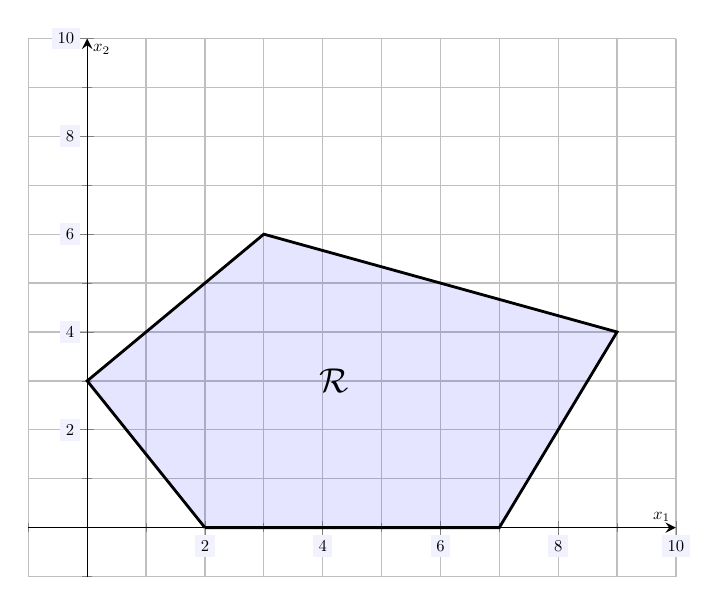
\begin{tikzpicture}[scale=1.2,every node/.style={scale=0.5}]
	\begin{axis}[
	grid=both,
	axis lines=middle,
	ticklabel style={fill=blue!5!white},
	xmin= -1, xmax=10,
	ymin= -1, ymax=10,
	xtick={0,2,4,6,8,10},
	ytick={0,2,4,6,8,10},
	minor tick = {-1,0,1,...,10},
	xlabel=\(x_1\),ylabel=\(x_2\),
	]
	\draw[line width=0.01cm,fill= blue,opacity=0.1] (2,0) -- (0,3) -- (3,6) -- (9,4) -- (7,0) -- (2,0);
	\draw[line width=0.03cm] (2,0) -- (0,3) -- (3,6) -- (9,4) -- (7,0) -- (2,0);
	\node at (4.2,3) {\huge$\mathcal{R}$};
	\end{axis}
	\end{tikzpicture}
	}
	\] \pspace

\sol Observe that the function $z= 5x_1 - 6x_2$ is linear in $x_1, x_2$. The region $\mathcal{R}$ is nonempty and bounded. Therefore, the Fundamental Theorem of Linear Programming states that $z$ must have a maximum and minimum value on $\mathcal{R}$ and these values occurs at a corner point for $\mathcal{R}$. So we need only evaluate $z$ at the corner points of $\mathcal{R}$. \par
	\begin{table}[H]
	\centering
	\begin{tabular}{cl}
	Corner Point & $z(x_1, x_2)$ \\ \hline
	$(2, 0)$ & $z(2, 0)= 5(2) - 6(0)= 10 - 0= 10$ \\
	$(7, 0)$ & $z(7, 0)= 5(7) - 6(0)= 35 - 0= 35$ \\
	$(9, 4)$ & $z(9, 4)= 5(9) - 6(4)= 45 - 24= 21$ \\
	$(3, 6)$ & $z(3, 6)= 5(3) - 6(6)= 15 - 36= -21$ \\
	$(0, 3)$ & $z(0, 3)= 5(0) - 6(3)= 0 - 18= -18$
	\end{tabular}
	\end{table}
Therefore, the maximum value for $z$ is $35$ and occurs at $(7, 0)$ and the minimum value for $z$ is $-21$ and occurs at $(3, 6)$. 



\newpage



% Problem 2
\problem{10} Consider the function $z= -3x_1 + 8x_2$ on the region $\mathcal{R}$ shown below. Does $z$ have a maximum or minimum value on $\mathcal{R}$? Explain. If the function has a maximum or minimum value on $\mathcal{R}$, find the maximum and minimum value. 
	\[
	\fbox{
	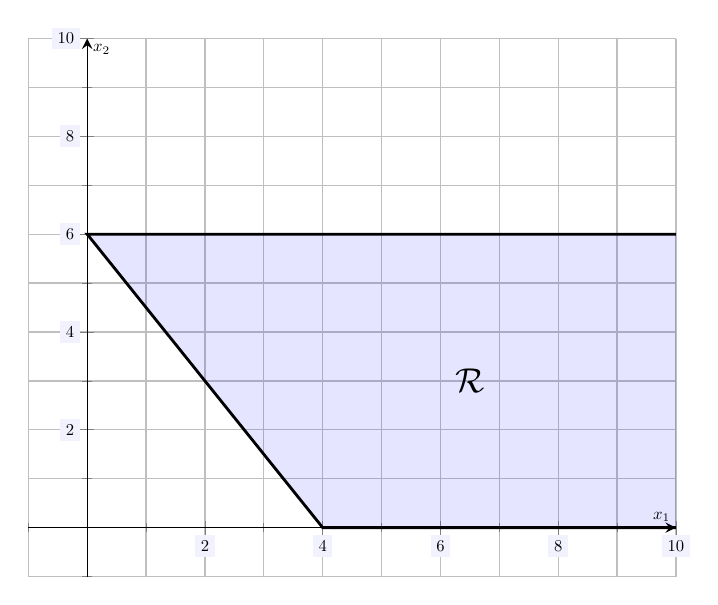
\begin{tikzpicture}[scale=1.2,every node/.style={scale=0.5}]
	\begin{axis}[
	grid=both,
	axis lines=middle,
	ticklabel style={fill=blue!5!white},
	xmin= -1, xmax=10,
	ymin= -1, ymax=10,
	xtick={0,2,4,6,8,10},
	ytick={0,2,4,6,8,10},
	minor tick = {-1,0,1,...,10},
	xlabel=\(x_1\),ylabel=\(x_2\),
	]
	
	\draw[line width=0.01cm,fill= blue,opacity=0.1] (4,0) -- (2,3) -- (0,6) -- (10,6) -- (10,0) -- (4,0);
	\draw[line width=0.03cm] (10,0) -- (4,0) -- (2,3) -- (0,6) -- (10,6);
	\node at (6.5,3) {\huge$\mathcal{R}$};
	\end{axis}
	\end{tikzpicture}
	}
	\] \pspace

\sol The function $z= -3x_1 + 8x_2$ is linear in $x_1, x_2$. The region $\mathcal{R}$ is nonempty. However, the region $\mathcal{R}$ is unbounded. Therefore, the Fundamental Theorem of Linear Programming does not apply. There may or may not be a maximum or minimum value for $z$ on $\mathcal{R}$. \pspace

Observe that the larger the value of $x_1$, the smaller the value of $z$. If $(x_1, x_2)$ is a point in the region $\mathcal{R}$, increasing $x_1$ moves the point to the right. But there is no limit on how far one can move to the point $(x_1, x_2)$ in $\mathcal{R}$ to the right and remain in $\mathcal{R}$. Therefore, there is no limit to how much one can decrease $z$. This shows that $z$ has no minimum value. \pspace

Observe that increasing $x_1$, i.e. decreasing $x_1$ increases $z$, and increasing $x_2$ increases $z$. If $(x_1, x_2)$ is a point in the region $\mathcal{R}$, decreasing $x_1$ moves the point to the left and increasing $x_2$ moves the point upwards. However, there is a limit to how much one can move a point upwards and to the left and stay in the region. Therefore, $z$ has a maximum value and it must occur at the point $(0, 6)$. The maximum value of $z$ is then $z(0, 6)= -3(0) + 8(3)= 0 + 24= 24$. 



\newpage



% Problem 3
\problem{10} Consider the function $z= x_1 - 9x_2$ on the region $\mathcal{R}$ shown below. Does $z$ have a maximum or minimum value on $\mathcal{R}$? Explain. If the function has a maximum or minimum value on $\mathcal{R}$, find the maximum and minimum value. 
	\[
	\fbox{
	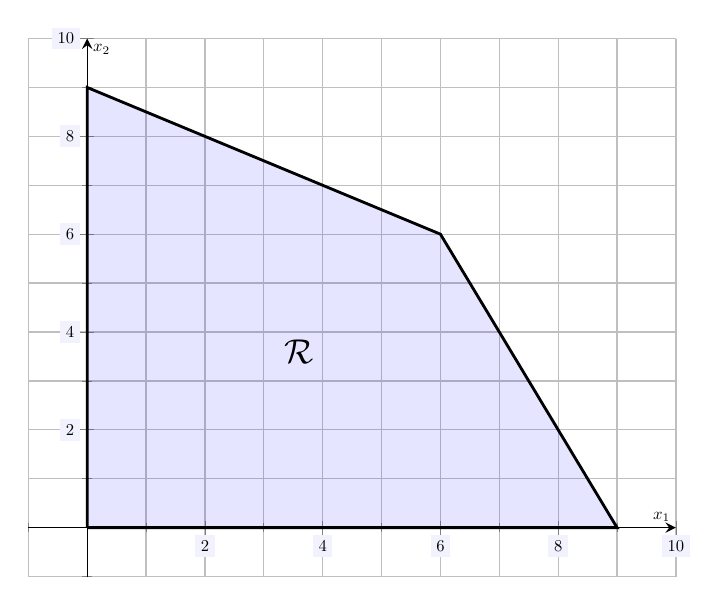
\begin{tikzpicture}[scale=1.2,every node/.style={scale=0.5}]
	\begin{axis}[
	grid=both,
	axis lines=middle,
	ticklabel style={fill=blue!5!white},
	xmin= -1, xmax=10,
	ymin= -1, ymax=10,
	xtick={0,2,4,6,8,10},
	ytick={0,2,4,6,8,10},
	minor tick = {-1,0,1,...,10},
	xlabel=\(x_1\),ylabel=\(x_2\),
	]
	\draw[line width=0.01cm,fill= blue,opacity=0.1] (0,0) -- (0,9) -- (6,6) -- (9,0) -- (0,0);
	\draw[line width=0.03cm] (0,0) -- (0,9) -- (6,6) -- (9,0) -- (0,0);
	\node at (3.6,3.6) {\huge$\mathcal{R}$};
	\end{axis}
	\end{tikzpicture}
	}
	\] \pspace

\sol The function $z= x_1 - 9x_2$ is linear in $x_1, x_2$. The region $\mathcal{R}$ is nonempty and bounded. By the Fundamental Theorem of Linear Programming, the function $z$ has a maximum and minimum value on $\mathcal{R}$ and occurs at a corner point of $\mathcal{R}$. So we need only evaluate $z$ at the corner points of $\mathcal{R}$. \par
	\begin{table}[H]
	\centering
	\begin{tabular}{cl}
	Corner Point & $z(x_1, x_2)$ \\ \hline
	$(0, 0)$ & $z(0, 0)= 0 - 9(0)= 0 - 0= 0$ \\
	$(9, 0)$ & $z(9, 0)= 9 - 9(0)= 9 - 0= 9$ \\
	$(6, 6)$ & $z(6, 6)= 6 - 9(6)= 6 - 54= -48$ \\
	$(0, 9)$ & $z(0, 9)=0 - 9(9)= 0 - 81= -81$
	\end{tabular}
	\end{table}
Therefore, the maximum value for $z$ is $9$ and occurs at $(9, 0)$ and the minimum value for $z$ is $-81$ and occurs at $(0, 9)$. 



\newpage



% Problem 4
\problem{10} Find the dual problem for the minimization problem shown below.
	\[
	\begin{gathered}
	\min w= 4y_1 + 6y_2 - 9y_3 \\
	\begin{cases}
	7y_1 + 3y_2 + 8y_3 \geq 37 \\
	4y_1 - y_2 + 5y_3 \geq 55 \\
	y_1 - y_2 + 3y_3 \leq 18 \\
	y_1, y_2, y_3 \geq 0
	\end{cases}
	\end{gathered}
	\] \pspace

\sol First, we need every inequality to be of the form `$\geq$' an integer. We multiply both sides of the third inequality by $-1$ to place this inequality in this form. This gives us the following inequalities (ignoring the non-negativity inequalities):
	\[
	\begin{gathered}
	\begin{cases}
	7y_1 + 3y_2 + 8y_3 \geq 37 \\
	4y_1 - y_2 + 5y_3 \geq 55 \\
	-y_1 + y_2 - 3y_3 \geq -18
	\end{cases}
	\end{gathered}
	\]
We then form a matrix $M$ from these inequalities with the function $w= 4y_1 + 6y_2 - 9y_3$ as the bottom row. This gives us the following matrix: 
	\[
	M=
	\begin{pmatrix}
	7 & 3 & 8 & 37 \\
	4 & -1 & 5 & 55 \\
	-1 & 1 & -3 & -18 \\
	4 & 6 & -9 & 0 
	\end{pmatrix}
	\]
We then compute the transpose of this matrix:
	\[
	M^T= 
	\begin{pmatrix}
	7 & 4 & -1 & 4 \\
	3 & -1 & 1 & 6 \\
	8 & 5 & -3 & -9 \\
	37 & 55 & -18 & 0 
	\end{pmatrix}
	\]
This is the `matrix of coefficients' for the inequalities for the corresponding dual maximization problem---the bottom row representing the function. The dual problem is a maximization problem so that the inequalities are `$\leq$.' Because there are $4$ columns, there are $4 - 1= 3$~variables in this system. [The last column corresponds to the `opposite' side of the inequalities.] Therefore, the dual maximization problem is\dots
	\[
	\begin{gathered}
	\max z= 37x_1 + 55x_2 - 18x_3 \\
	\begin{cases}
	7x_1 + 4x_2 - x_3 \leq 4 \\
	3x_1 - x_2 + x_3 \leq 6 \\
	8x_1 + 5x_2 - 3x_3 \leq -9 \\
	x_1, x_2, x_3 \geq 0
	\end{cases}
	\end{gathered}
	\] 


\end{document}